\documentclass[11pt]{article}

\usepackage[margin=0.75in]{geometry}
\usepackage{amsfonts, amsmath, amssymb}
\usepackage[none]{hyphenat}
\usepackage{fancyhdr}
\usepackage{graphicx}
\usepackage{float}
\usepackage[nottoc, notlot, notlof]{tocbibind}

%matlab code packages
\usepackage{listings}
\usepackage{color} %red, green, blue, yellow, cyan, magenta, black, white
\definecolor{mygreen}{RGB}{28,172,0} % color values Red, Green, Blue
\definecolor{mylilas}{RGB}{170,55,241}

\pagestyle{fancy}
\fancyhead{}
\fancyfoot{}
\fancyhead[L]{Engineering Mathematics(course 25735)}
\fancyhead[R]{Reza Nayeb Habib 401102694}
\fancyfoot[C]{\thepage}
\fancyfoot[R]{Sharif University of Technology}
\renewcommand{\footrulewidth}{1pt}
\parindent 0ex

\begin{document}

\lstset{language=Matlab,%
    %basicstyle=\color{red},
    breaklines=true,%
    morekeywords={matlab2tikz},
    keywordstyle=\color{blue},%
    morekeywords=[2]{1}, keywordstyle=[2]{\color{black}},
    identifierstyle=\color{black},%
    stringstyle=\color{mylilas},
    commentstyle=\color{mygreen},%
    showstringspaces=false,%without this there will be a symbol in the places where there is a space
    numbers=left,%
    numberstyle={\tiny \color{black}},% size of the numbers
    numbersep=9pt, % this defines how far the numbers are from the text
    emph=[1]{for,end,break},emphstyle=[1]\color{red}, %some words to emphasise
    %emph=[2]{word1,word2}, emphstyle=[2]{style},    
}
    
\begin{titlepage}
\begin{center}

\begin{figure}[H]
\begin{center}

\includegraphics[scale=0.4]{Fig/SUT.png}

\end{center}
\end{figure}

\huge{\textbf{Engineering Mathematics Project Report}} \\ 
\vspace*{2cm}
\Large{\textbf{Instructor: Prof. Karbalaei}} \\
\vspace*{1cm}
\huge{\textbf{Sharif University of Technology}} \\
\line(1,0){500} \\ 
\Huge{\textbf{Magnetic Resonance Imaging (MRI) Reconstruction from K-Space}} \\
\line(1,0){500} \\
\vfill
\Large{By Reza Nayeb Habib}\\
\Large{Student ID\# 401102694} \\

\end{center}
\end{titlepage}

\tableofcontents
\thispagestyle{empty}
\clearpage
\setcounter{page}{1}

\section{Introduction}
\section{MRI and K-Space}
\subsection{Question 1} 
\textbf{Explain the concept of 2D Fourier transform. What are the bases of the 2D Fourier trans-
form?} \\
In fourier transform we had:
$$ F(\omega) = \int_{-\infty}^{+\infty} f(x) e^{-j 2 \pi \omega x}\, dx$$
now using the same idea in a 2D space, 2D fourier transform is defined as:
$$ F(u,v) = \int_{-\infty}^{+\infty} f(x,y) e^{-j 2 \pi (ux + vy)}\, dxdy$$
the basis of 2D fourier is u (or in K-Space $\mathrm{K}_x$) which is the frequency in x axis,
and v (or in K-Space $\mathrm{K}_y$) which is the frequency in y axis.

\subsection{Question 2}
\textbf{What is the connection between each point in k-space and raw image? What does each
point in k-space represent?} \\
the value of each point $(\mathrm{K}_x,\mathrm{K}_y)$ in K-Space represents the intensity of that frequency
in the raw image.

\subsection{Question 3}
\textbf{Consider the images below:} \\
\begin{figure}[H]
    \begin{center}
        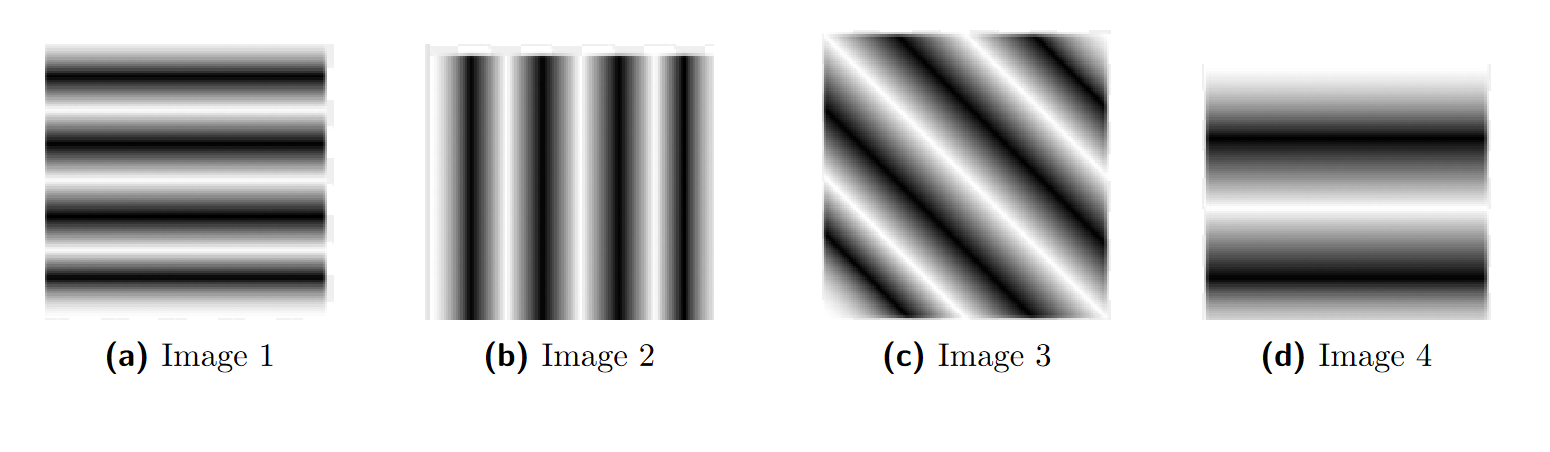
\includegraphics[scale=0.5]{Fig/2.3.kspace.images.png}
    \end{center}
\end{figure}
\textbf{We transform each image into k-space, each point in the plot below represents one of the images
in the k-space. For each picture, select the correct point in the k-space.} \\
we showed the corresponding image to the corresponding points in figure \ref*{fig:kspaceAxis}

\begin{figure}[H]
\begin{center}
    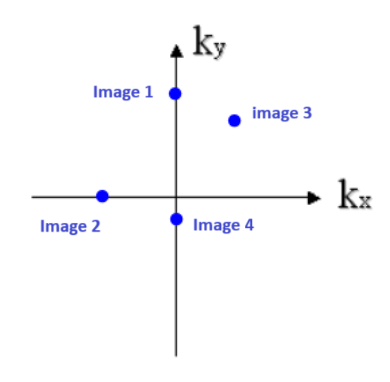
\includegraphics[scale=0.8]{Fig/2.2kspace.axis.png}
    \label{fig:kspaceAxis}
    \caption{Images on their corresponding points on K-Space}
\end{center}
\end{figure}
we can see that Image 1 looks like the function $\sin(y)$ and both Images 2 and 4 look like $\sin(x)$
and the third image is like $\sin(x+y)$ function.

\subsection{Question 4}
\textbf{Consider the MRI image and its k-space transformed image below:} \\
\begin{figure}[H]
    \begin{center}
        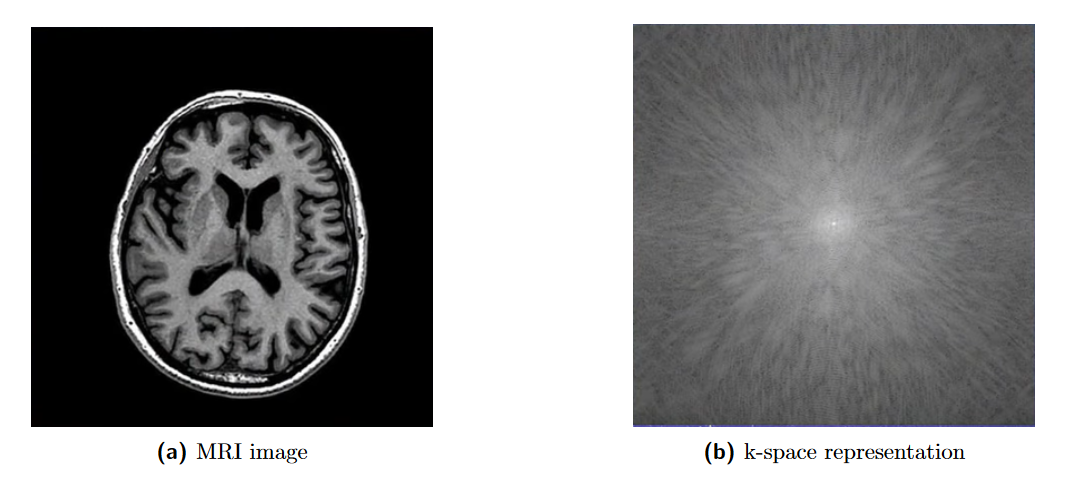
\includegraphics[scale=0.5]{Fig/Q1-4.png}
    \end{center}
\end{figure}
\textbf{What happens if we delete high-frequency bases in k-space? what about low-frequency
bases? which one would preserve the original image more?} \\
\begin{figure}[H]
    \begin{center}
        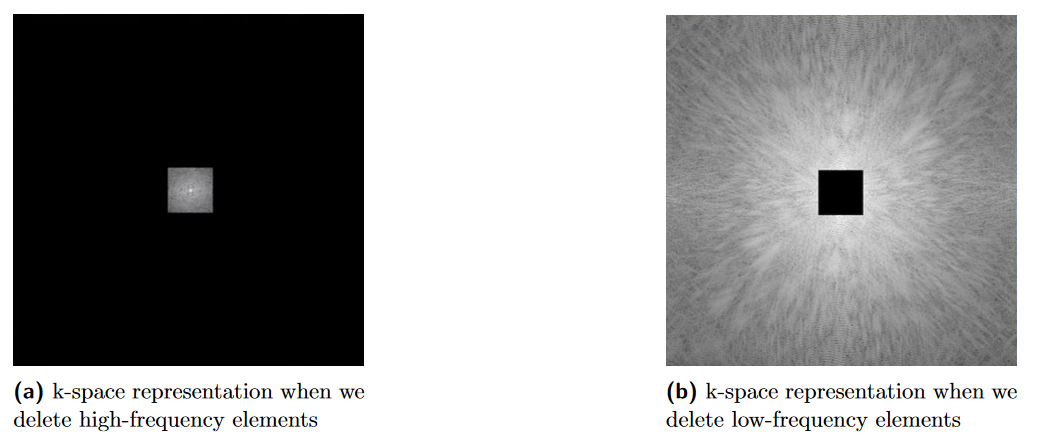
\includegraphics[scale=0.5]{Fig/Q1-4-1.png}
    \end{center}
\end{figure}
it can be seen that the low-frequency bases in K-Space have more intensity in their color
this means they store more data than high-frequency bases thus we can conclude that removing
high-frequency bases preserves the image better than removing low-frequency bases. 

\section{MRI Reconstruction}

\subsection{Question 1}
\textbf{For the purpose of this project, search and explain two of the above-mentioned methods
for MRI Reconstruction from k-space data.} \\
\vspace{0.2cm} \\
\textbf{FBP:} in this method we backpropagate the pixel from it's nearest neighbors
on the sensor and from the direction the wave source emmits its waves to our detector.
FBP (Filtered Back Projection) reconstruction method helps create 2D or 3D images from MRI data. This process involves two key steps. First, 
the acquired data goes through a filter. This filter emphasizes certain 
details while reducing noise. Then, the filtered data is back-projected to form the image. The back projection spreads
the filtered data back into the image space, revealing the structure of the imaged object. This method is often used in 
MRI, especially in cases where the data is collected in a radial or spiral trajectory. Though widely used, FBP has limitations, particularly 
in complex MRI acquisition scenarios. In those cases, iterative reconstruction methods such as SENSE and GRAPPA are often preferred for better image quality.
\vspace{1cm} \\
\textbf{Parallel imaging}: Parallel imaging is a technique in MRI that uses multiple receiver coils to accelerate 
image acquisition. By leveraging information from multiple coils, parallel imaging reduces 
the amount of data that needs to be acquired, thereby shortening scan times or 
improving image resolution. Two popular parallel imaging techniques are SENSE (Sensitivity Encoding) 
and GRAPPA (Generalized Autocalibrating Partial Parallel Acquisitions).


\subsection{Question 2}
\textbf{Load the rawkneedata.mat that is attached to this file.} \\
\lstinputlisting{Code/loading.m}
\subsection{Question 3}
\textbf{Reconstruct the MRI image using a 2D-inverse Fourier transform. Explain your method.}\\
\lstinputlisting{Code/reconstruction.m}
we first do a 2D inverse fourier transform on the raw data with MATLAB ifft2() function,
then we shift the image using fftshift to get the correct inverse fourier and finally we show it with imshow.
\subsection{Question 4}
\textbf{Plot the reconstructed MRI.} \\
\vspace{0.2cm} \\
\begin{figure}[H]
    \begin{center}
        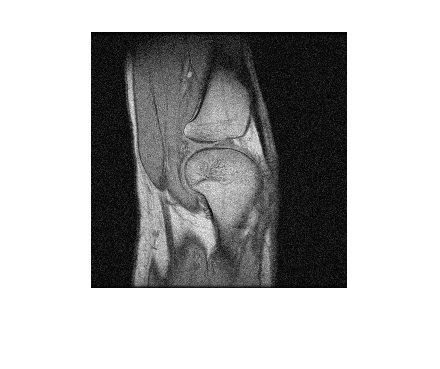
\includegraphics[scale=0.8]{Fig/ifft2.knee.png}
        \label{fig:noisyImage}
        \caption{Reconstructed MRI picture using ifft2}
    \end{center}
\end{figure}


\subsection{Question 5}
\textbf{Can you observe the noises available in your reconstructed MRI? Discuss briefly the noises
in medical images, and in particular MRI images..} \\
\vspace{0.1cm} \\

the noise in the picture can be seen especially the white spots in the darker areas. \\
Generally it is common for MRI images to contain noise due to the method they are
created(emmiting waves wich can cause us receiving unwanted signals from the emitter device).
also detectors can have inaccuracies and the environment can also cause some noise,
thus noise reduction is important for obtaining useful medical images that can be used
for treating medical conditions.

\section{Metrics}
\subsection{Histogram}
\textbf{Use the matplotlib.pyplot.hist in Python on imhist in MATLAB commands to display the
histograms of the noisy and noiseless images. Explain the characteristics of the filter used to
reduce noise in the frequency domain based on the two histograms obtained. Is it a high-pass,
middle-pass, or low-pass filter?} \\
\begin{figure}[H]
    \begin{center}
        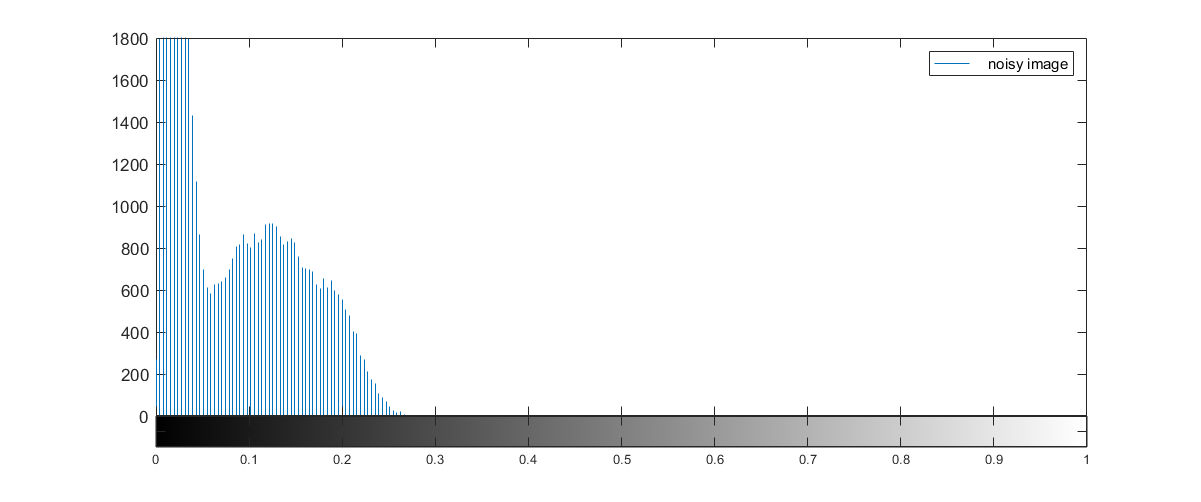
\includegraphics[scale=0.5]{Fig/noisy.hist.png}
        \label{fig:noisyHist}
        \caption{Histogram of the noisy image}
    \end{center}
\end{figure}

\begin{figure}[H]
    \begin{center}
        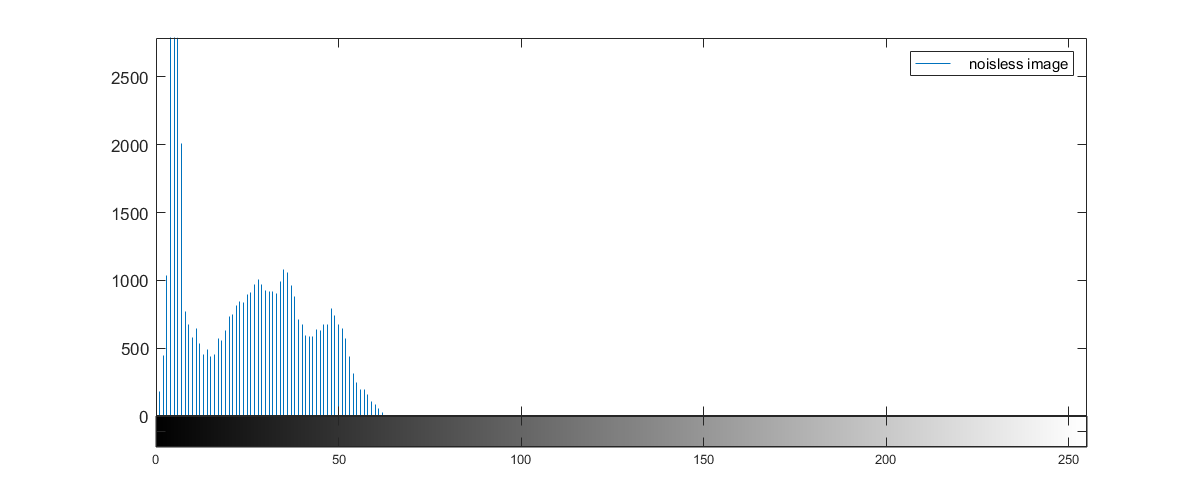
\includegraphics[scale=0.5]{Fig/noisless.hist.png}
        \label{fig:noislessHist}
        \caption{Histogram of the noiseless image}
    \end{center}
\end{figure}
by looking at the histograms we can conclude that the filter used is more like a middle pass on that has reduced both low
frequency bases and high frequency ones.

\subsection{Low Pass Filters} 
\textbf{We want to reduce image noise by applying spatial filters. Read carefully about the Mean,
median, and Gaussian filters, and briefly explain each in your report.} \\
\vspace{5pt} \\
\textbf{Mean Filter:} this method convolves a matrix with size nxn
with all elements being $\frac{1}{\mathrm{n}}$. this method is technicaly just
taking the mean of all of the neighbors(and the pixel itself) of the pixel and replacing the
pixel with the mean value thus being names Mean Filter.(See \ref{fig:MeanFlt}) \\
\begin{figure}[H]
    \begin{center}
        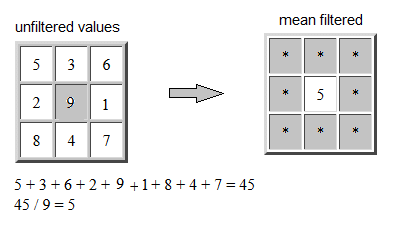
\includegraphics[scale=0.6]{Fig/Mean.filter.png}
        \label{fig:MeanFlt}
        \caption{the working of a mean filter}
    \end{center}
\end{figure}
\textbf{Median filter:} this method chooses an nxn matrix of the pixels neighborhood
and chooses the mean between those pixels(see \ref{fig:MedianFlt}) \\
\begin{figure}[H]
    \begin{center}
        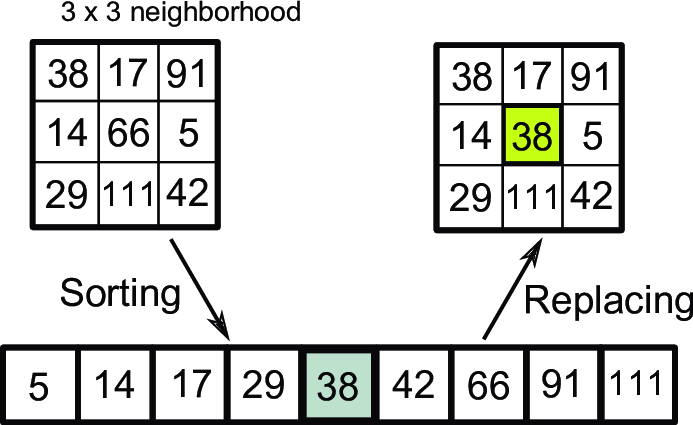
\includegraphics[scale=0.35]{Fig/Median.filter.png}
        \label{fig:MedianFlt}
        \caption{the working of a median filter}
    \end{center}
\end{figure}

\textbf{Gaussian Filter:} for applying the Gaussian Filter we first create a kernel matrix
in the shape of a gaussian distribution, with formula:
$$G_{2D}(X,Y,\sigma) = \frac{1}{2\pi \sigma^2}e^{-\frac{X^2+Y^2}{2 \sigma^2}}$$
where X and Y are nxn matrices with shape:
$$ X = 
\begin{bmatrix}
    -\left[\frac{n}{2}\right] & -\left[\frac{n}{2}\right]+1 & ... & 0 & ... & \left[\frac{n}{2}\right]-1 & \left[\frac{n}{2}\right] \\
    ... & ... & ... & 0 & ... & ... & ...\\
    -\left[\frac{n}{2}\right] & -\left[\frac{n}{2}\right]+1 & ... & 0 & ... & \left[\frac{n}{2}\right]-1 & \left[\frac{n}{2}\right] \\
\end{bmatrix}$$
$$Y = 
\begin{bmatrix}
    -\left[\frac{n}{2}\right] &  ... & -\left[\frac{n}{2}\right]\\
    -\left[\frac{n}{2}\right]+1 &  ... & -\left[\frac{n}{2}\right]+1 \\
    ... & ... & ... \\
    0 & 0 & 0 \\
    ... & ... & ... \\
    \left[\frac{n}{2}\right]-1 &  ... & \left[\frac{n}{2}\right]-1 \\
    \left[\frac{n}{2}\right] & ... & \left[\frac{n}{2}\right] \\
\end{bmatrix}
$$
after creating the kernel we convolve it with our image.

\subsection{Mean Filter}
\textbf{Write a function that applies a Mean filter to an input image and returns the filtered image.
You are not allowed to use any pre-built Mean filter functions.7 (kernel size is up to you.)} \\
\lstinputlisting{Code/meanflt2.m}
\begin{figure}[H]
    \begin{center}
        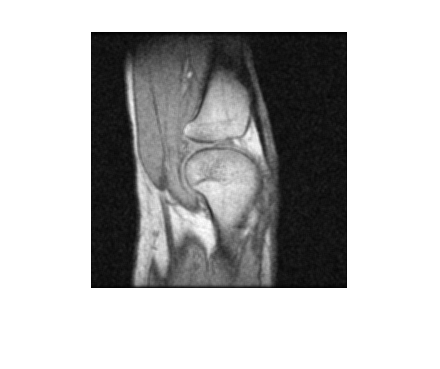
\includegraphics[scale=0.6]{Fig/mean.knee.png}
        \label{fig:MeanKnee}
        \caption{filtered image using Mean Filter}
    \end{center}
\end{figure}
\subsection{Median Filter}
\textbf{Write a function that, upon receiving the kernel size, applies the median filter to the input
image and returns the filtered image. (Hint: Use scipy.signal.medfilt in Python or medfilt2 in
MATLAB)} \\

\lstinputlisting{Code/medianflt2.m}
\begin{figure}[H]
    \begin{center}
        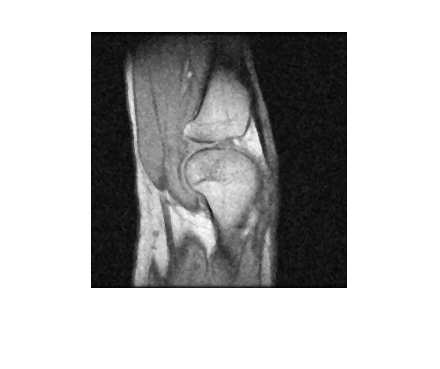
\includegraphics[scale=0.6]{Fig/median.knee.png}
        \label{fig:MedianKnee}
        \caption{filtered image using Median Filter}
    \end{center}
\end{figure}
\subsection{Gaussian Filter}
\textbf{Write a function that applies a Gaussian filter to an input image and returns the filtered
image. You are not allowed to use any pre-built Mean filter functions.6 (kernel size is up to
you.)} \\
\lstinputlisting{Code/gaussianflt2.m}
\begin{figure}[H]
    \begin{center}
        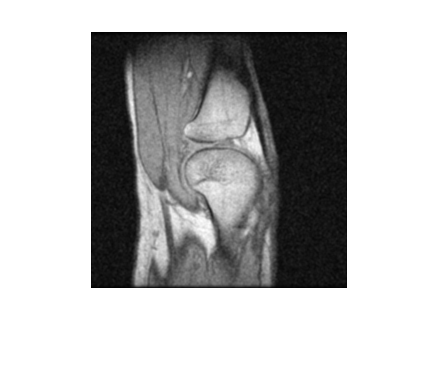
\includegraphics[scale=0.6]{Fig/gaussian.knee.png}
        \label{fig:GaussianKnee}
        \caption{filtered image using Gaussian Filter}
    \end{center}
\end{figure}
\subsection{Non-Local Means}
\textbf{The non-local means (NLM) noise reduction algorithm is well known as an excellent tech-
nique for removing noise from a magnetic resonance (MR) image to improve diagnostic accu-
racy. [5] Research this algorithm and describe its method. Then reduce the noise of the image
using the pre-built functions imnlmfilt in MATLAB or skimage.restoration.denoise-nl-means in
Python.} \\
\vspace{5pt} \\
Non-Local Means algorithm gets a weighted sum over all pixels in the image,
weighted by how similar two pixels are together, unlike unlike local Mean(Mean Filter discussed in 4.3)
which gets the mean of the pixels close to the target pixel. the formula for this weighted sum is as follows. \\
consider the pixels $p$ and $q$, the set of all pixels in the image shown by $\Omega$
function $u(p)$ which gives the filtered value of point $p$ then we have($v(q)$ is the unfiltered value of $q$):
$$  u(p) = \frac{1}{C(p)}\int_{\Omega} v(q)f(p,q)dq $$
where $f(p,q)$ is the weight function denoting the similarity of $p$ and $q$ and $C(p)$ is the normalizing factor.
the $C(p)$ normalizing factor is also given by:
$$ C(p) = \int_{\Omega}f(p,q)dq $$
unlike the normalizing favtor the weighting functions isn't unique
and various formulas can be used for it but one of the commonly used functions is
the Gaussian weighting function:
$$ f(p, q) = \exp -\frac{|B(q) - B(p)|^2}{h^2}$$
where $h$ is the filtering parameter(the standard deviation) and $B(p)$
is the local mean value of the image point values surrounding $p$.
\begin{figure}[H]
    \begin{center}
        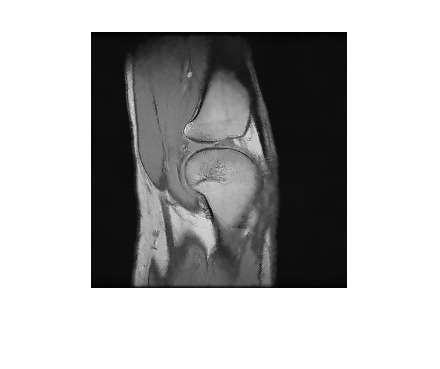
\includegraphics[scale=0.6]{Fig/non-local.mean.png}
        \label{fig:Non-LocalKnee}
        \caption{filtered image using Non-Local Mean Filter}
    \end{center}
\end{figure}


\subsection{Evaluation}
\textbf{Evaluate the output of the four methods discussed in this section using SNR and PSNR
criteria and present the results, compared with kneeMRI.jpeg in a table. Also, calculate these
two criteria for the initial noisy image and declare which method performed better in noise
reduction.} \\
\lstinputlisting{Code/SNR.m}

by coding the given algorithms in matlab we derived the following table:
\begin{figure}[H]
    \begin{center}
        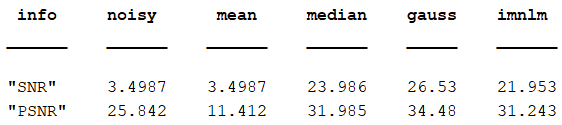
\includegraphics[scale=1]{Fig/eval.png}
        \label{fig:Evaluation}
    \end{center}
\end{figure}
wich shows that the Gaussian and Local-Mean are the best filters and the mean filter
is the worst. \\
by looking at the pictures by eye we can see that although the SNR and PSNR of the Gaussian and Loacal-Mean
are close the Local-Mean gives better resoloution so that may be the reason it is prefered for use in MRI denoising.

\end{document}